\section{\scshape kNN}

\subsection{Ogólne informacje}
\begin{frame}{Ogólne informacje}
	\begin{itemize}
	\item Metoda nieparametryczna.
	\item Wykorzystywany do:
	\begin{itemize}
		\item klasyfikacji;
		\item prognozowania warto"sci zmiennej losowej (regresja).
	\end{itemize}
	\end{itemize}
\end{frame}

\subsection{Uczenie maszynowe}
\begin{frame}{Uczenie maszynowe}
	\begin{itemize}
	\item Uczenie z przykładów (\emph{instance-based learning}).
	\item Wnioskowanie bezpo"srednio na podstawie zbioru uczącego.
	\item Złożono"sć ro"snie wraz z rozmiarem danych.
	\end{itemize}
\end{frame}

\begin{frame}{Faza uczenia się}
\begin{itemize}
	\item Zbiory uczące są wektorami przestrzeni wielowymiarowej.
	\item Faza uczenia polega tylko na zapamiętaniu danych.
	\item Niski koszt.
\end{itemize}
\end{frame}

\subsection{Opis algorytmu}
\begin{frame}{Dobór parametru}
\begin{itemize}
	\item Zdefiniowanie stałej \emph{k}.
	\item \emph{k} odpowiada z liczbę analizowanych sąsiadów.
	\item Większe warto"sci redukują wypływ szumu na klasyfikację.
\end{itemize}
\end{frame}

\begin{frame}{Opis algorytmu}
\begin{itemize}
	\item Wektory zbioru uczącego posiadają etykietę.
	\item Klasyfikacja obiektu poprzez znalezienie najczę"sciej pojawiającej się etykierty w"sród \emph{k} sąsiadów.
	\begin{center}
	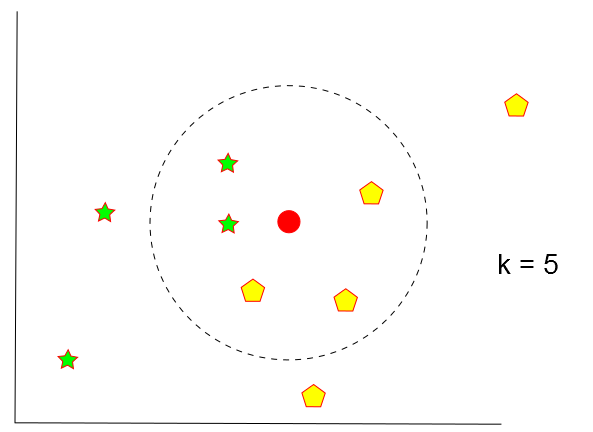
\includegraphics[keepaspectratio=true, scale=0.3]{neigh_small}
	\end{center}
	\item Odległo"sć od sąsiada okre"sla się na podstawie odpowiedniej metryki.
\end{itemize}
\end{frame}

\begin{frame}{Różne k}
	\begin{center}
	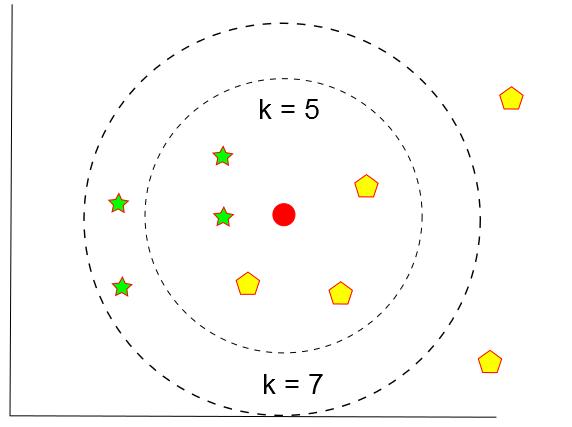
\includegraphics[keepaspectratio=true, scale=0.55]{neigh_k_small}
	\end{center}
\end{frame}
